\documentclass[conference]{IEEEtran}
\usepackage{amsmath,amssymb}
\usepackage{graphicx}
\usepackage{booktabs}
\usepackage{url}
\usepackage{multirow}
\usepackage{cite}

\graphicspath{{figures/}}

\begin{document}

\title{Workload-Aware Long-Range Link Selection for Physically Constrained Chiplet Networks}

\author{
\IEEEauthorblockN{Lobna Ghanim}
\IEEEauthorblockA{Advanced Topics in Hardware Accelerators for Deep Learning --- Course Project Report}
}

\maketitle

\begin{abstract}
Two-dimensional mesh networks are simple and regular, but distant chiplets may communicate through several hops. This project evaluates whether a small number of physically feasible long-range links can reduce that cost, and whether choosing those links for the current workload is more effective than freezing a workload-independent topology. A 16-chiplet, $4\times4$ mesh was extended with up to $K \in \{1,2,4\}$ shortcuts under total wire budgets of $5$, $15$, $25$, and $45$~mm. Selection minimizes analytical workload-average latency while preserving the original workload's maximum directed-link-load bound and enforcing wire, topology, and PHY constraints. RapidChiplet~\cite{rapidchiplet} provides physical and analytical evaluation; regenerated shortest-path routes are validated with the BookSim cycle-accurate simulator~\cite{booksim}. Tests cover random-uniform, transpose, permutation, and hotspot synthetic traffic, plus three distributed-training traces (\texttt{gpt\_pipeline}, \texttt{gpt\_fsdp}, \texttt{moe\_expert}) generated with STAGE~\cite{stage} and converted into chiplet traffic matrices.

Across 48 synthetic workload/budget/$K$ configurations, Workload-Aware links reduce mean low-load BookSim latency by $12.039\%$ relative to a fair 8-PHY Mesh baseline and by $5.792\%$ relative to a Fixed (workload-independent) shortcut baseline. Across 36 STAGE configurations the corresponding means are $5.545\%$ and $2.150\%$. Workload-Aware beats Mesh in 78/84 configurations and Fixed in 55/84; Fixed nevertheless wins 5/36 STAGE cases. The strongest observed advantage over Fixed is $24.752\%$ (synthetic transpose, $B{=}45$~mm, $K{=}1$). Requesting more links frequently installs no additional link ($\mathrm{actual\_k} < \mathrm{requested\_k}$ in 28/48 synthetic and 18/36 STAGE Workload-Aware configurations). The results support workload-aware shortcut selection as a useful, workload-dependent design point rather than a universally superior topology.
\end{abstract}

\section{Introduction}

Chiplet-based (multichiplet) integration disaggregates a monolithic die into smaller, reusable dies connected through a package-level interconnect, improving yield, cost, and design reuse for large-scale DNN and LLM accelerators~\cite{simba}. This modularity, however, shifts the architectural burden onto the inter-chiplet network: as systems scale to more chiplets, communication distance and hop count grow, and the choice of topology and routing becomes a first-order performance and energy factor.

\subsection{Problem domain and existing approaches}
A two-dimensional mesh is the dominant choice for network-on-chip (NoC) and network-on-package (NoP) interconnects because it is hardware-friendly, regular, and simple to route with dimension-order routing~\cite{hire}. Its principal weakness is that hop count -- and therefore latency and energy -- grows with network diameter. Chen~\emph{et al.}~\cite{hire} quantify this directly: on a SIMBA-based~\cite{simba} $2$D-mesh multichiplet accelerator, weak-scaling the network-on-package from $2\times2$ to $8\times8$ chiplets increases average latency by $3.4\times$ and degrades energy efficiency by $7.1\times$ under ResNet-50 and OPT-6.7B workloads. Several works address this by introducing long-range \emph{bypass} links that shortcut the mesh: Kite~\cite{kite} enumerates a family of heterogeneous interposer topologies constructed by adding bypass links to a base mesh and models their interconnect properties analytically; HiRe~\cite{hire} introduces hierarchical \emph{reconfigurable nodes} (RNs) on an active silicon interposer that dynamically switch bypass connections at runtime, combined with an offline simulated-annealing communication scheduler and a greedy, provably deadlock-free path-selection routing algorithm, reporting $14.3$--$45.2\%$ energy-delay-product (EDP) reduction and $14.1$--$35.0\%$ latency reduction over five state-of-the-art fixed and reconfigurable baselines (SIMBA~\cite{simba}, NN-Baton, NSF-FT, INDM~\cite{indm}, Adapt-NoC). Other systems, such as INDM~\cite{indm}, co-design the interconnect network and the DNN dataflow mapping for a fixed topology chosen once at design time.

These works establish two important, but distinct, points: (i) long-range links meaningfully reduce hop count and communication cost on top of a mesh, and (ii) making the network \emph{reconfigurable} so that link usage can adapt to the running dataflow yields a further gain over any single fixed topology. HiRe achieves adaptability through \emph{circuit-level runtime reconfiguration} of active-interposer switches, which requires dedicated reconfigurable-node hardware, an online 4-step reconfiguration protocol, and an offline simulated-annealing scheduler whose runtime grows from $\sim$12~minutes to $\sim$4.3~hours as the network scales from $2\times2$ to $8\times8$.

\subsection{Drawbacks addressed and project contribution}
This project asks a narrower, complementary question: rather than making the hardware reconfigurable at runtime, can a \emph{small, fixed number of long-range shortcut links, chosen once at design time for the anticipated workload}, already capture most of the available benefit under a strict, physically grounded resource budget (wire length, spare PHY endpoints, and no regression in worst-case link load)? This targets three practical drawbacks of runtime reconfiguration: (1) reconfigurable nodes and their control logic add area/power/verification cost even when idle; (2) the SA-based scheduler in \cite{hire} requires nontrivial offline compute and per-workload re-tuning; and (3) many deployed accelerator packages cannot add active reconfiguration logic to the interposer at all, but \emph{can} afford a handful of extra static long-range wires and PHY endpoints decided once, analogous to Kite's~\cite{kite} static topology family.

Concretely, this project builds on the RapidChiplet toolchain~\cite{rapidchiplet} -- an open-source physical/analytical chiplet design-space exploration framework from ETH Z\"urich's Scalable Parallel Computing Lab (no associated publication; cited here as software) -- and the BookSim cycle-accurate interconnection-network simulator~\cite{booksim} for validation. On top of this base infrastructure we implement:
\begin{itemize}
\item an exhaustive, constraint-satisfying \emph{Workload-Aware} shortcut-link selector for $K{=}1$ requested links, and a greedy iterative extension for $K{=}2$ and $K{=}4$;
\item a \emph{Fixed} baseline that uses the identical selection machinery but conditions link choice on a workload-independent uniform-traffic reference, isolating the effect of workload awareness from the effect of adding shortcuts at all;
\item a converter that maps STAGE~\cite{stage}-generated distributed-training communication traces (GPT pipeline-parallel, GPT fully-sharded data-parallel, and mixture-of-experts traffic) into RapidChiplet traffic matrices, so the same machinery can be evaluated on realistic LLM-training communication patterns rather than only synthetic traffic; and
\item a full physical-cost, multi-seed robustness, and reproducibility-audit analysis pipeline.
\end{itemize}

The central research question is:
\begin{quote}
\emph{Under equal physical resources, can workload-aware long-range chiplet links provide a better communication-performance tradeoff than a conventional mesh or a workload-independent fixed set of shortcuts?}
\end{quote}
Section~\ref{sec:methods} details the baseline architecture and the selection algorithm; Section~\ref{sec:impl} describes the experimental implementation; Section~\ref{sec:results} reports and discusses the results.

\section{Methods}
\label{sec:methods}

\subsection{Original approach: RapidChiplet baseline modeling}
RapidChiplet~\cite{rapidchiplet} represents a chiplet package as a set of JSON-described inputs -- chiplets (with PHY/link-endpoint geometry), a 2D placement, packaging parameters, a topology (graph of links between chiplet PHYs or interposer routers), and a routing table -- and computes, from these inputs, package area, chiplet/interposer/link power, manufacturing yield/cost, per-link Manhattan length and length-dependent latency and bandwidth, and two network-level metrics used throughout this project:
\begin{itemize}
\item \textbf{Analytical average latency} $L_{avg}(T,\text{topology})$: for a traffic matrix $T$ and a fixed routing table, the weighted-average end-to-end latency (in cycles) over all communicating chiplet pairs, accounting for source/destination router latency, PHY latency, per-hop relay latency, and per-link length-dependent latency.
\item \textbf{Directed link load}: for a given traffic matrix and routing, the aggregate traffic routed over each directed link; its maximum over all links, $\mathrm{MaxLoad}(T,\text{topology})$, is used as a peak-congestion proxy.
\end{itemize}
This project uses RapidChiplet's existing physical/analytical machinery unmodified and adds the workload-aware and fixed shortcut-selection algorithms, the STAGE traffic converter, and the comparison pipeline described below.

\subsection{Baseline architecture}
The evaluated network is a $4\times4$ mesh of 16 chiplets with 24 undirected nearest-neighbor links. The original 4-PHY design reserves exactly the four cardinal PHYs per chiplet needed for mesh connectivity and cannot host any shortcut without breaking a mesh edge. To make a fair Mesh-vs-Fixed-vs-Workload-Aware comparison possible, all three policies instead use an \textbf{8-PHY} chiplet: four cardinal PHYs (west/north/east/south) carry the mesh, and four spare PHYs are reserved for shortcuts. The no-shortcut 8-PHY mesh ($K{=}0$) is therefore the fair baseline against which both Fixed and Workload-Aware are measured, since all three policies share identical chiplet dimensions, placement, packaging, and PHY budget. Table~\ref{tab:phy-overhead} quantifies the capability cost of provisioning the four spare PHYs even when no shortcut is installed.

\begin{table}[t]
\centering
\caption{Capability overhead of 8-PHY vs.\ 4-PHY chiplets.}
\label{tab:phy-overhead}
\begin{tabular}{lccc}
\toprule
Metric & 4-PHY & 8-PHY & Increase \\
\midrule
Chiplet area (mm$^2$) & 77.400 & 80.800 & 4.393\% \\
Chiplet power (W) & 20.500 & 21.000 & 2.439\% \\
PHY count & 4 & 8 & +4 (100\%) \\
\bottomrule
\end{tabular}
\end{table}

\subsection{Workload-aware link-selection algorithm}
Let $T$ be a workload traffic matrix, $K$ the maximum number of shortcut links to add, $B$ the total wire budget, and $E_{extra}$ the selected shortcut set. The optimization is
\begin{equation}
\min_{E_{extra}} \; L_{avg}(T, E_{extra})
\end{equation}
subject to
\begin{align}
|E_{extra}| &\le K, \label{eq:c1}\\
\sum_{e \in E_{extra}} \mathrm{Length}(e) &\le B, \label{eq:c2}\\
\mathrm{MaxLoad}(T, E_{extra}) &\le \mathrm{MaxLoad}_{\text{baseline}}(T), \label{eq:c3}
\end{align}
together with feasibility constraints that every shortcut (i) connects a non-mesh chiplet pair, (ii) uses valid, currently unoccupied spare PHYs, and (iii) is not a duplicate of an existing mesh edge or already-selected shortcut. Constraint~(\ref{eq:c3}) is essential: it prevents the optimizer from trading a lower \emph{average} latency for a worse \emph{peak} bottleneck relative to the unmodified mesh under the same traffic.

\textbf{$K{=}1$ (exact).} The candidate set is all $\binom{16}{2} - 24 = 96$ non-mesh chiplet pairs. Each candidate is filtered by (\ref{eq:c2})--(\ref{eq:c3}) and scored by $L_{avg}$; the minimum-latency feasible candidate is selected, with load, length, and endpoint identifier used as deterministic tie-breakers. This is exact over the enumerated candidate model.

\textbf{$K{=}2,4$ (greedy).} Exhaustive combinatorial search over multi-link sets was not used; instead, the topology is extended one link at a time:
\begin{quote}\small
\texttt{selected = []; topology = mesh; occupied = mesh\_PHYs; remaining = B}\\
\texttt{for step in 1..K:}\\
\texttt{\quad feasible = []}\\
\texttt{\quad for each unused non-mesh pair (u,v):}\\
\texttt{\qquad pick shortest available spare-PHY pair}\\
\texttt{\qquad reject if length > remaining}\\
\texttt{\qquad add link, regenerate routing, evaluate}\\
\texttt{\qquad reject if max load > baseline max load}\\
\texttt{\qquad record candidate}\\
\texttt{\quad if feasible is empty: stop}\\
\texttt{\quad best = arg min latency (ties: load, length, id)}\\
\texttt{\quad commit best; mark PHYs occupied; remaining -= length}\\
\texttt{return selected  (actual\_k = len(selected) <= K)}
\end{quote}
Because the search is greedy, $\mathrm{actual\_k}$ can be, and frequently is, smaller than the requested $K$ when no further link satisfies (\ref{eq:c2})--(\ref{eq:c3}) or improves latency.

Routing after every permanent topology change is regenerated using RapidChiplet's deterministic shortest-path routing so that all reported metrics correspond to the actual, updated graph rather than a stale routing table.

\subsection{Fixed baseline}
\textit{Fixed} uses the identical selector, budgets, spare-PHY architecture, and max-load constraint, but is conditioned once on a uniform all-to-all reference traffic matrix and then frozen across every evaluated workload:
\begin{center}
\small
\begin{tabular}{ll}
Fixed: & uniform reference $\to$ choose once $\to$ freeze\\
Workload-Aware: & current workload $\to$ choose for that workload\\
\end{tabular}
\end{center}
This isolates \emph{traffic conditioning} as the only variable between the two policies -- both use the same physical candidate model, wire budgets, and constraints.

\section{Implementation and Experiments}
\label{sec:impl}

\subsection{What was reused vs.\ implemented}
\textbf{Reused as-is:} RapidChiplet's core physical/analytical engine (\texttt{rapidchiplet.py}, \texttt{helpers.py}, \texttt{validation.py}) for area, power, cost, link-length/latency/bandwidth, and analytical latency/throughput computation; RapidChiplet's BookSim export/import wrapper (\texttt{booksim\_wrapper.py}) and the vendored BookSim~2 simulator~\cite{booksim}; and the STAGE trace generator~\cite{stage} for producing distributed-training Chakra execution traces.

\textbf{Implemented for this project:} the $K{=}1$ exhaustive and $K{=}2/4$ greedy Workload-Aware selectors; the Fixed selector variants; the physical-baseline (4-PHY vs.\ 8-PHY) generator; a from-scratch Chakra-protobuf trace inspector and a STAGE-to-RapidChiplet traffic converter (with explicit send/receive pairing, ring-based collective expansion for \texttt{ALL\_REDUCE}/\texttt{ALL\_GATHER}/\texttt{REDUCE\_SCATTER}/\texttt{ALL\_TO\_ALL}, and normalization to the synthetic traffic scale); the synthetic multi-seed workload generator; all Mesh/Fixed/Workload-Aware BookSim run drivers; the policy-comparison, physical-cost, multi-seed, and final-analysis scripts; and a stored-artifact reproducibility auditor.

\subsection{Experimental configuration}
The factorial design covers wire budgets $B \in \{5,15,25,45\}$~mm, requested link counts $K \in \{1,2,4\}$, and eight workloads: four synthetic (\texttt{random\_uniform}, \texttt{transpose}, \texttt{permutation}, \texttt{hotspot}) and three STAGE-derived (\texttt{gpt\_pipeline}: DP=2,TP=2,PP=4; \texttt{gpt\_fsdp}: DP=16 with FSDP; \texttt{moe\_expert}: DP=2,TP=2,EP=4), each with 16 ranks mapped one-to-one onto the 16 chiplets. \texttt{permutation} and \texttt{hotspot} are additionally regenerated for seeds $42$--$46$ for robustness. Every Fixed/Workload-Aware topology starts from the same 24-link 8-PHY mesh; the exact selected chiplet/PHY endpoints are inserted and routing is regenerated, so workload traffic is the only variable that changes between Fixed designs sharing a $(K,B)$ point.

For each resulting design, RapidChiplet screening records analytical average latency, aggregate throughput, maximum directed-link load, wire length, and length-dependent link latency; BookSim validation then records the low-load packet latency (the smallest complete numeric offered-load point), average hop count, accepted rate, and a full offered-load sweep, from which we derive the \textbf{derived latency knee}: the first tested offered load at which average packet latency reaches at least twice the low-load latency. This is an empirical threshold over tested points, not an exact analytical throughput boundary, and is reported only where available rather than being extrapolated.

STAGE traces were generated with compact but representative model/parallelism configurations (16 ranks each) chosen so that the resulting Chakra traces exercise pipeline point-to-point traffic (\texttt{gpt\_pipeline}), FSDP all-gather/reduce-scatter collectives (\texttt{gpt\_fsdp}), and expert-parallel all-to-all traffic (\texttt{moe\_expert}); converted traffic totals $69{,}140{,}480$, $269{,}352{,}960$, and $270{,}188{,}544$ bytes of network communication respectively, spanning 56, 16, and 80 nonzero chiplet pairs. All three conversions were validated end-to-end (re-parsed trace vs.\ stored inventory, byte-conservation of the ring expansion, and RapidChiplet schema validation of the generated traffic files).

\section{Results and Discussion}
\label{sec:results}

\subsection{$K{=}1$: exact selection}
Table~\ref{tab:k1-transpose} shows the strongest single result in the study: for \texttt{transpose} at $B{=}45$~mm, Workload-Aware selects the single link $3{\leftrightarrow}12$ (41.35~mm), reducing low-load latency from Mesh's 98.863 to 71.543 cycles (a $27.634\%$ gain) and from Fixed's 95.076 to 71.543 cycles (a $24.752\%$ gain), while average hop count falls from 4.316 to 3.164.

\begin{table}[t]
\centering
\caption{Transpose, $K{=}1$: Mesh vs.\ Fixed vs.\ Workload-Aware.}
\label{tab:k1-transpose}
\small
\begin{tabular}{lccccc}
\toprule
$B$ (mm) & Mesh & Fixed & Aware & Aware wire & Gain vs.\ Fixed\\
\midrule
5  & 98.863 & 98.863 & 85.717 & 4.794  & 13.298\% \\
15 & 98.863 & 90.463 & 81.738 & 13.933 & 9.645\%  \\
25 & 98.863 & 95.076 & 73.339 & 23.072 & 22.863\% \\
45 & 98.863 & 95.076 & 71.543 & 41.350 & 24.752\% \\
\bottomrule
\end{tabular}
\end{table}

Notably, the $B{=}45$ configuration has the lowest low-load latency but a \emph{lower} derived knee ($0.037$) than Mesh's ($0.042$), i.e., the best low-load latency point need not be the best point under increasing offered load -- these are related but distinct notions of ``better.''

\begin{figure}[t]
\centering
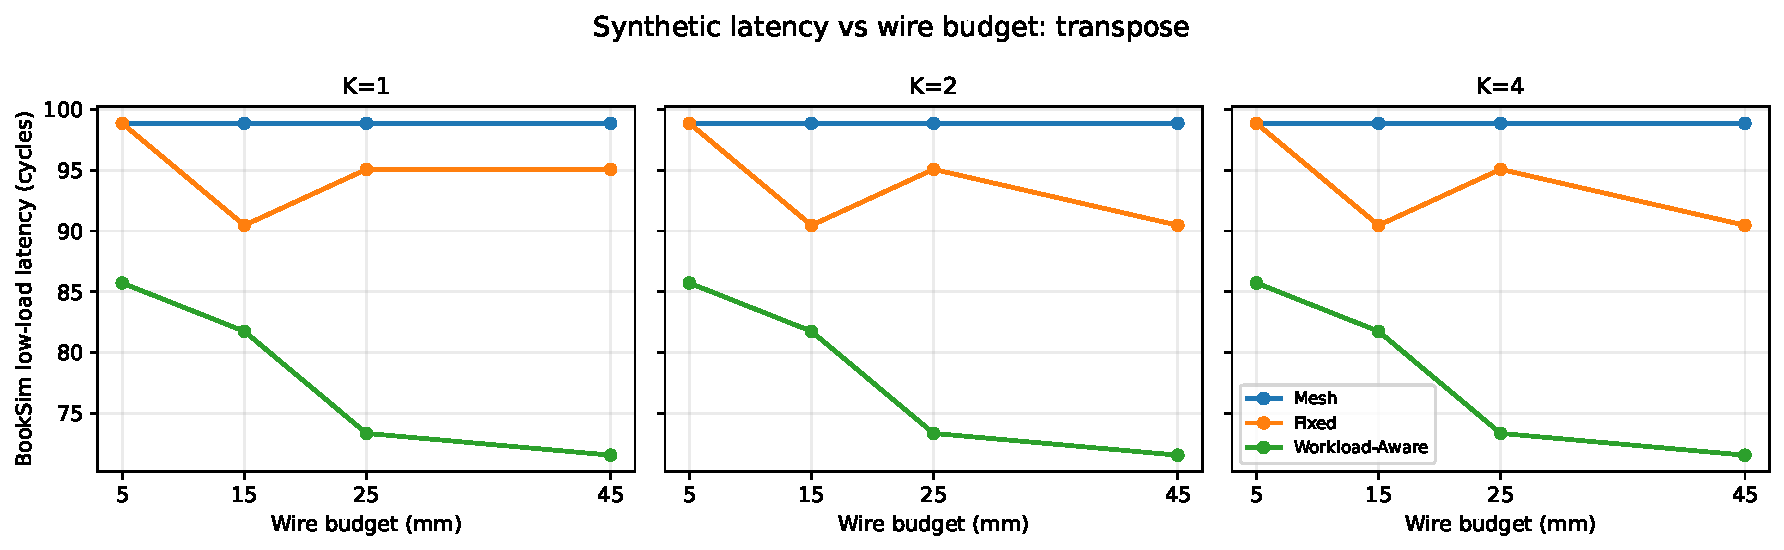
\includegraphics[width=\linewidth]{synthetic_latency_vs_budget_transpose.pdf}
\caption{Transpose low-load latency vs.\ physical wire budget. Workload-specific placement outperforms the uniform-reference Fixed topology at every budget.}
\label{fig:transpose}
\end{figure}

For \texttt{random\_uniform}, Workload-Aware reproduces Fixed exactly at every $K$ and $B$, as expected since Fixed is itself conditioned on a uniform-traffic reference -- this is an internal consistency check on the selectors, not a separate result.

\subsection{Effect of requested $K$}
Table~\ref{tab:k-summary} aggregates all 16 synthetic workload/budget points at each requested $K$. Increasing $K$ gives diminishing returns: mean Workload-Aware latency falls only from 77.247 (K=1) to 76.395 (K=2) to 75.958 cycles (K=4), while mean \emph{installed} links rises just from 1.000 to 1.188 to 1.375. Across 32 successive $K$-transitions per policy, 27/32 Workload-Aware and 28/32 Fixed transitions changed latency by no more than $0.1\%$ and added no link at all -- constraints (\ref{eq:c2})--(\ref{eq:c3}) and PHY/candidate availability, not the requested $K$, are usually the binding factor. Figure~\ref{fig:actual-k} shows this directly: $\mathrm{actual\_k} < \mathrm{requested\_k}$ in 28/48 synthetic Fixed and 28/48 Workload-Aware configurations.

\begin{table}[t]
\centering
\caption{Synthetic results aggregated by requested $K$ (16 workload/budget points each).}
\label{tab:k-summary}
\small
\begin{tabular}{lcccc}
\toprule
$K$ & Mean Aware & Gain vs.\ Mesh & Gain vs.\ Fixed & Mean $\mathrm{actual\_k}$ \\
\midrule
1 & 77.247 & 11.192\% & 5.589\% & 1.000 \\
2 & 76.395 & 12.205\% & 5.602\% & 1.188 \\
4 & 75.958 & 12.719\% & 6.186\% & 1.375 \\
\bottomrule
\end{tabular}
\end{table}

\begin{figure}[t]
\centering
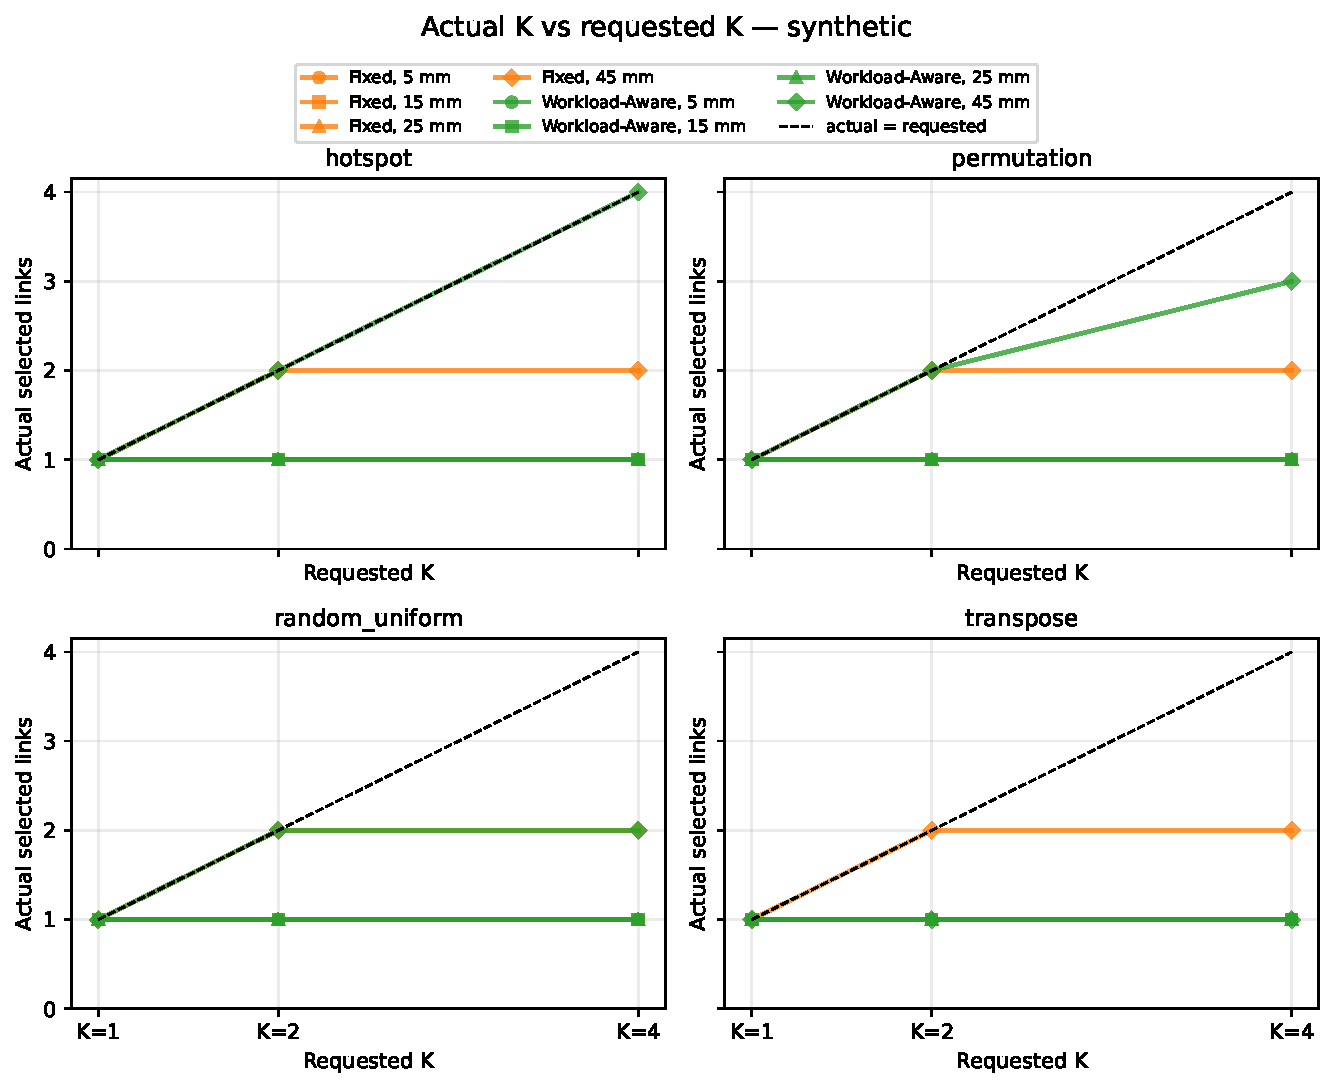
\includegraphics[width=\linewidth]{actual_k_vs_requested_k_synthetic.pdf}
\caption{Installed vs.\ requested $K$ (synthetic workloads). Selection frequently stops before the requested budget of links is used.}
\label{fig:actual-k}
\end{figure}

\subsection{Multi-seed robustness}
\texttt{permutation} and \texttt{hotspot} were regenerated for five random seeds ($42$--$46$) to separate the persistence of the \emph{performance gain} from the repeatability of the \emph{exact topology chosen}. As Fig.~\ref{fig:multiseed} shows, every seed group retains a positive Workload-Aware gain (mean $9.831\%$ for permutation, $8.239\%$ for hotspot; observed group minimum $3.246\%$), while the exact selected topology is much less stable -- groups contain 2--5 distinct topologies, and the modal topology occurs in only $35$--$37\%$ of seeds on average. This indicates the \emph{benefit} of workload-aware selection is robust to random traffic instantiation even though the specific chosen link is not.

\begin{figure}[t]
\centering
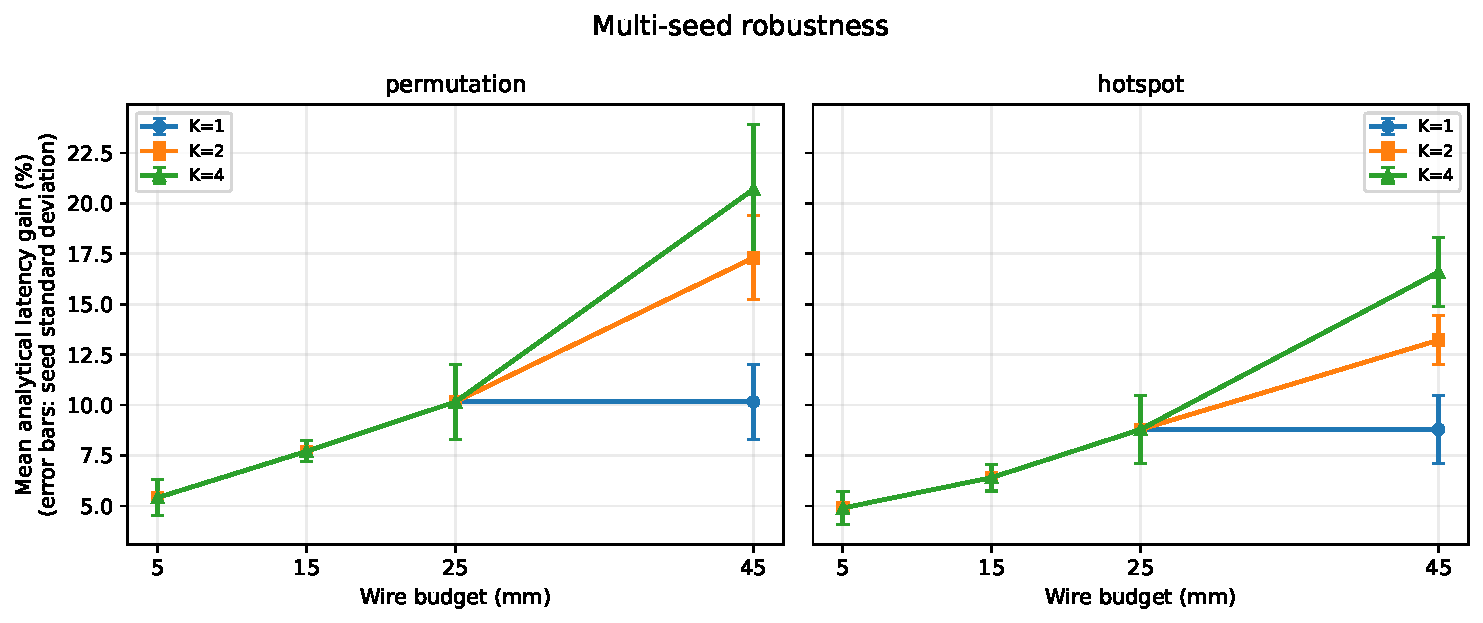
\includegraphics[width=\linewidth]{multiseed_latency_gain_robustness.pdf}
\caption{Latency-gain robustness across seeds 42--46 for permutation and hotspot.}
\label{fig:multiseed}
\end{figure}

\subsection{STAGE-derived (distributed-training) workloads}
Table~\ref{tab:stage} averages the three STAGE workloads at every $(B,K)$ point. Workload-Aware still wins on average, but by a substantially smaller margin than on synthetic traffic (mean $5.545\%$ vs.\ Mesh, $2.150\%$ vs.\ Fixed, over 36 configurations), and it is not universal: \texttt{gpt\_fsdp} at $B{=}45$, $K{=}2/4$ is a clear counterexample, where Fixed's two-link topology reaches 47.019 cycles versus Workload-Aware's one-link 50.166 cycles ($-6.693\%$). The strongest STAGE gains are for \texttt{gpt\_pipeline} at $B{=}45,K{=}4$ ($11.428\%$ over Fixed) and \texttt{moe\_expert} at the same point ($10.988\%$).

\begin{table}[t]
\centering
\caption{STAGE workloads, mean over three traces per $(B,K)$ point.}
\label{tab:stage}
\small
\begin{tabular}{cccccc}
\toprule
$B$ & $K$ & Mesh & Fixed & Aware & Gain vs.\ Fixed\\
\midrule
5  & 1--4 & 50.596 & 50.048 & 50.047 & 0.001\% \\
15 & 1--4 & 50.596 & 48.099 & 48.354 & $-0.387\%$ \\
25 & 1 & 50.596 & 48.982 & 47.352 & 3.358\% \\
25 & 2,4 & 50.596 & 48.982 & 46.311 & 5.583\% \\
45 & 1 & 50.596 & 48.982 & 46.789 & 4.416\% \\
45 & 2 & 50.596 & 47.053 & 45.748 & 2.773\% \\
45 & 4 & 50.596 & 47.053 & 44.587 & 5.241\% \\
\bottomrule
\end{tabular}
\end{table}

\begin{figure}[t]
\centering
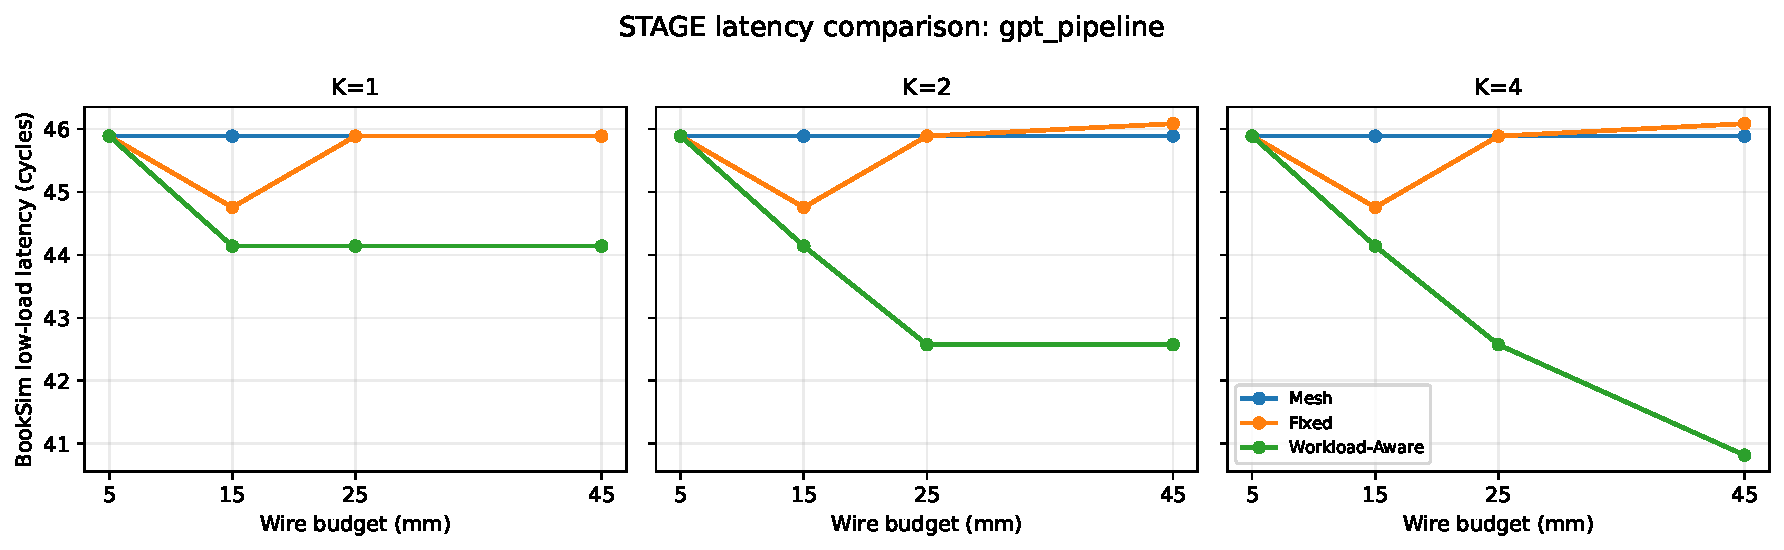
\includegraphics[width=\linewidth]{stage_latency_comparison_gpt_pipeline.pdf}
\caption{GPT-pipeline latency comparison: gains from workload-aware selection grow with wire budget.}
\label{fig:gpt-pipeline}
\end{figure}

The broad synthetic conclusion therefore generalizes only in qualified form: workload conditioning usually helps real distributed-training communication patterns too, particularly at larger budgets, but a uniform-reference topology can occasionally match or beat the workload-specific analytical choice, especially when a workload (e.g., FSDP all-gather/reduce-scatter, which is largely symmetric) does not deviate much from the uniform assumption used to pick Fixed.

\subsection{Physical-cost analysis}
Capability cost (the 8-PHY provisioning of Table~\ref{tab:phy-overhead}) is paid regardless of usage; usage cost depends on the selected configuration. Across all 168 Fixed/Workload-Aware logical configurations, mean added wire is 18.635~mm, mean $\mathrm{actual\_k}$ is 1.208, and mean spare-PHY utilization is only $3.776\%$ of the 64 available spare endpoints (Fig.~\ref{fig:physical-wire}). Mean descriptive efficiency is 0.483 latency-gain percentage points per mm of wire and 0.403 hop-gain points per mm. Only two $K$-transitions added wire for negligible or negative latency gain, both of which \emph{worsened} latency -- reflecting that greedy analytical selection, physical link latency, and BookSim's cycle-accurate behavior are related but not identical objectives.

\begin{figure}[t]
\centering
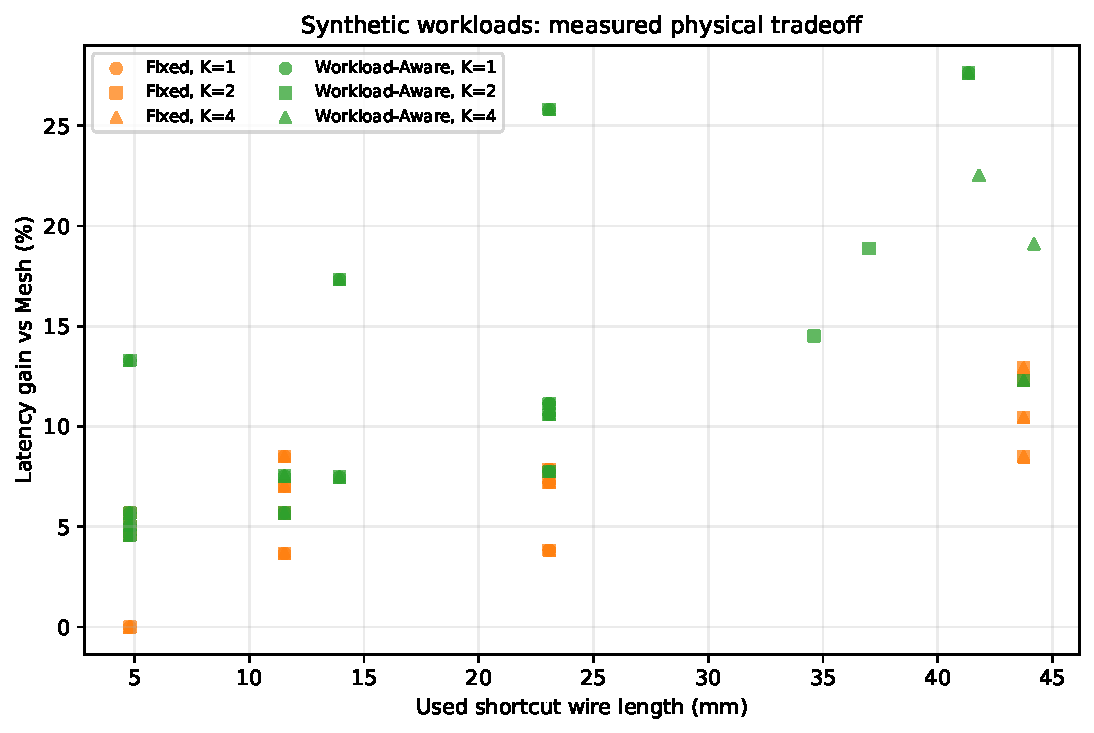
\includegraphics[width=\linewidth]{synthetic_latency_gain_vs_physical_wire.pdf}
\caption{Latency gain vs.\ physical wire used. More wire expands the feasible topology space, but gain per millimeter varies substantially by workload and policy.}
\label{fig:physical-wire}
\end{figure}

\subsection{Discussion}
Workload-aware links help most when traffic has structure the uniform reference does not capture: transpose shows a $17.000\%$ average advantage over Fixed versus $0\%$ for random-uniform (an exact tie by construction). Fixed is competitive precisely when the workload resembles the uniform reference, when the budget only admits the same short candidate regardless of traffic, or when a fixed topology happens to serve a particular realistic workload (e.g., \texttt{gpt\_fsdp}) well. Budget is an upper bound, not a spending target: mean synthetic Workload-Aware wire rises from 4.794~mm at $B{=}5$ to 36.531~mm at $B{=}45$ while mean gain vs.\ Mesh rises from $7.156\%$ to $17.668\%$, yet identical topologies can persist across adjacent budgets, and a longer selected link can even reduce the derived knee. The maximum-directed-link-load constraint (\ref{eq:c3}) is what prevents the optimizer from buying a lower average latency at the cost of a worse peak bottleneck; together with finite spare PHYs and greedy candidate availability, this is the main reason $\mathrm{actual\_k}$ is so often below $\mathrm{requested\_k}$.

Relative to HiRe's~\cite{hire} runtime-reconfigurable approach, the design-time static shortcut selection studied here achieves a smaller but still substantial fraction of the available benefit ($5$--$28\%$ latency gains depending on workload, vs.\ HiRe's $14.1$--$35.0\%$ over fixed \emph{and} reconfigurable state-of-the-art baselines) without any online reconfiguration hardware, control protocol, or per-run scheduling cost -- consistent with the two approaches occupying different points on the adaptability/complexity tradeoff curve rather than being directly substitutable.

\subsection{Limitations}
The architecture is limited to a $4\times4$, 16-chiplet network, and scaling trends were not measured directly (cf.\ HiRe's~\cite{hire} weak-scaling study to $8\times8$). $K{>}1$ selection is greedy, not globally exhaustive, so a locally optimal prefix may exclude a better joint combination. All comparisons use one deterministic shortest-path routing scheme; alternative or adaptive routing (e.g., HiRe's greedy path selection~\cite{hire}) could change both load and latency. Workloads are static traffic-matrix abstractions that do not model temporal phases, compute/network overlap, or reconfiguration delay. STAGE conversion assumes a one-to-one rank-to-chiplet mapping and a ring-based collective expansion policy read directly from STAGE's own configuration. Only three STAGE workloads and five random seeds (for two of four synthetic workloads) were evaluated. The derived latency knee is a first-crossing empirical threshold, not a formal congestion boundary, and analytical screening and BookSim validation are related but not identical models.

\subsection{Future work}
Natural extensions include evaluating larger chiplet arrays and alternative spare-PHY organizations; combining static shortcut selection with HiRe-style~\cite{hire} adaptive or congestion-aware routing; replacing the greedy $K{>}1$ selector with a global or combinatorial optimizer to quantify the greedy optimality gap; and modeling reconfiguration latency, control overhead, and reliability explicitly if link selection were made runtime-adaptive rather than fixed at design time. Phase-aware STAGE optimization (choosing different links per collective phase rather than one aggregated matrix) and evaluation on additional LLM parallelism configurations would further test the generality of the STAGE result.

\subsection{Conclusion}
Under a fair, equal-PHY-budget comparison, Workload-Aware long-range links generally outperform both a plain mesh (78/84 configurations, mean gains of $12.039\%$ synthetic / $5.545\%$ STAGE) and a workload-independent Fixed baseline (55/84 configurations, mean gains of $5.792\%$ synthetic / $2.150\%$ STAGE) -- but not universally: Fixed wins 5/36 STAGE cases, and increasing the requested link budget $K$ gives strongly diminishing returns because physical and load-preservation constraints, not link count, are usually the binding factor. The answer to the research question is \emph{yes, in general for this tested system, but conditionally}: workload-aware shortcut selection is a useful, workload-dependent design point that must be co-designed with wire budget, PHY availability, and peak-load protection rather than maximized independently.

\begin{thebibliography}{9}

\bibitem{rapidchiplet}
P.~Iff \emph{et al.}, ``RapidChiplet,'' Scalable Parallel Computing Laboratory (SPCL), ETH Z\"urich. [Software]. Available: \url{https://github.com/spcl/rapidchiplet}

\bibitem{booksim}
N.~Jiang, D.~U.~Becker, G.~Michelogiannakis, J.~Balfour, B.~Towles, J.~Kim, and W.~J.~Dally, ``A Detailed and Flexible Cycle-Accurate Network-on-Chip Simulator,'' in \emph{Proc. IEEE Int. Symp. Performance Analysis of Systems and Software (ISPASS)}, 2013.

\bibitem{stage}
C.~Man, J.~Park, H.~Wu, H.~Xu, S.~Sridharan, and T.~Krishna, ``Scalable Synthesis of Distributed LLM Workloads through Symbolic Tensor Graphs,'' in \emph{Proc. 53rd Annu. Int. Symp. Comput. Archit. (ISCA)}, 2026. arXiv:2511.10480.

\bibitem{hire}
Z.~Chen, J.~Zhang, D.~Lyu, H.~Chen, J.~Jiang, W.~Sheng, C.~Zhang, and G.~He, ``HiRe: A Hierarchical Reconfigurable Architecture for Large-Scale Multichiplet DNN Accelerators,'' \emph{IEEE Trans. Very Large Scale Integr. (VLSI) Syst.}, vol.~34, no.~6, pp.~1736--1749, Jun. 2026.

\bibitem{simba}
B.~Zimmer \emph{et al.}, ``A 0.32--128 TOPS, Scalable Multi-Chip-Module-Based Deep Neural Network Inference Accelerator With Ground-Referenced Signaling in 16 nm,'' \emph{IEEE J. Solid-State Circuits}, vol.~55, no.~4, pp.~920--932, Apr. 2020.

\bibitem{kite}
S.~Bharadwaj, J.~Yin, B.~Beckmann, and T.~Krishna, ``Kite: A Family of Heterogeneous Interposer Topologies Enabled via Accurate Interconnect Modeling,'' in \emph{Proc. 57th ACM/IEEE Design Autom. Conf. (DAC)}, 2020.

\bibitem{indm}
J.~Zhang \emph{et al.}, ``INDM: Chiplet-Based Interconnect Network and Dataflow Mapping for DNN Accelerators,'' \emph{IEEE Trans. Comput.-Aided Design Integr. Circuits Syst.}, vol.~43, no.~4, pp.~1107--1120, Apr. 2024.

\end{thebibliography}

\end{document}
